\chapter{System implementation}

In this chapter I will discuss the actual implementation of the original idea
behind Linkero: a brand monitoring case management application. I will start
from the architecture in order to show a general snapshot of the system, before
talking in details about every single component, the technology that was
chosen and reasons behind. I will follow with use cases and
system requirements, to conclude with class diagram, database structure and some
code samples.

\section{Development challenge}
They system architecture described in the next session \emph{System
architecture} needs a little explanation, because it deviates from the standard
three-tier architecture of many websites.

Before this project I already developed a stand-alone, single thread,
application that would generate reports of eBay items and sellers. The
application was written in Python and included a simple user interface,
corresponding to what is now the eBay input form (see figure
\ref{fig:inputform}). The application would take the user input, retrieve the
data using eBay public API and would create and save in the local hard-drive a
csv file. It was all that was needed, and worked well for one single user that
needed access only to eBay data.

More users and new features immediately showed the limits of the stand-alone
application approach:
\begin{itemize}
  \item the installation process was not straight forward for non-technical
  users, since a Python version needed to be installed along with some other
  non-standard libraries and dependencies;
  \item some sort of version control system needed to be established and
  maintained in order to guarantee that all users would run the latest version.
\end{itemize}

The idea of a web-application seemed the perfect solution for those two issues:
\begin{itemize}
  \item there would be no need to install the application locally, since every
  user could just use the tool by simply logging in onto the website;
  \item every user would be aligned on the latest version, since any new
  feature would be implemented on the server and immediately available to
  everyone.
\end{itemize}

However a centralized server calling external data-sources on behalf of
different, potentially concurrent, clients created a different set of
challenges. Online services who open up their database to external users via
API, normally limit the number of requests a single user can make in two ways:
\begin{itemize}
  \item total number of requests per user (e.g. 10,000 API calls each user);
  \item total number of requests per period (e.g. 100 API calls each minute).
\end{itemize}

API users need to register to a \emph{developer program} and they need to
include a API key in their GET or POST requests parameters, this way the data
controller (who owns the data) can control the number of requests submitted by
each member. A work-around solution could have been to request each user to
register an API key for each service they wished to access and save their API key in
Linkero's profile settings, so that each user was directly responsible for
his/her own API calls quota. But it seemed a step-back from the original idea of
insulating the user from lower-level inner workings of the application.

The other issue emerging from the web-application approach, related to the time
the system takes to complete a report. eBay API results from a text search
are paginated, and each page returns a maximum of 100 items, over a maximum of
100 pages. There are a total of 22 country sites where the same search can be
repeated. After the search is completed we still need to retrieve the item
details, which is done with a different API. Long story short: a report
returning the maximum amount of results on all 22 eBay sites can take as long
as 15 hours to complete, if requests are sequential and the transmission lag
between request and response is half a second long. While a stand alone
application could run for as long as needed, while the user runs other programs,
you could not ask the user of a web application to keep the tab open until the
request is completed.

The solution I came up with is inspired by the \emph{broker pattern}: the broker
is a component of the system that coordinates communications between different
decoupled components \cite{JB00}. In Linkero, the broker is the part of the
application that takes data requests coming from different clients, and returns
a \emph{report submitted} response to the client, so that the client knows
his/her report has been scheduled and will receive a notification when it is
ready, meanwhile the user can close the browser windows or request other
reports. The broker on the other end, will queue the request and a single unit
will then process every report in the queue sequentially, thus avoiding to
exceed API call request limits with concurrent requests.

In the next section I will discuss how this architecture was implemented in
practice.

\section{System architecture}
The system architecture represented in figure \ref{fig:sysarch} provides an
overview of all different applications that work together to perform the main
system functionalities.

\begin{figure}[h!]
\centering
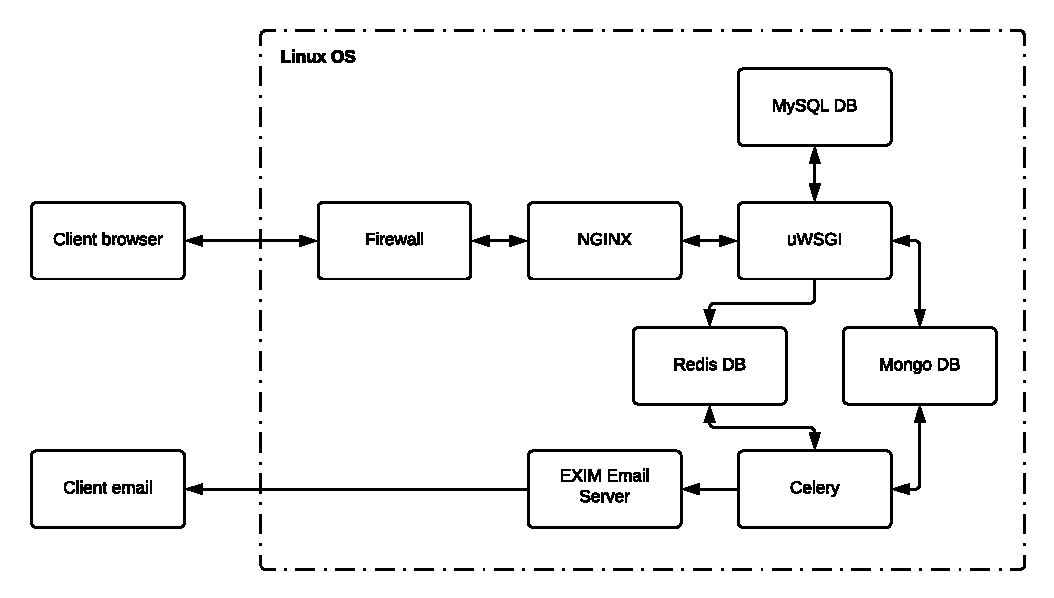
\includegraphics[scale=0.7]{imgs/SystemArchitecture.pdf}
\caption{Linkero system architecture}
\label{fig:sysarch}
\end{figure}

As shown in the figure, client browser and client email are considered part of
the system: the browser is included because some functionalities are passed to
the client to run locally in the form of JQuery functions, and the client email
is considered part of the system, because it represents the final destination of
data files generated by the system.

Linux is the operating system running on a Virtual Private Server, that manages
all other applications. The first point of entry is the Firewall, which monitors
all requests knocking on ports 22, 80 and 443.

NGINX is the web server, reverse proxy server \cite{WikiNginx}, which receives
HTTP requests and assigns them to the correct internal web server.

uWSGI is the web engine that runs Python scripts, in the words of its
developers: ``uWSGI itself is a vast project with many components, aiming to
provide a full software stack for building hosting services'' \cite{RtduWsgi}.

Python scripts from within uWSGI can make calls to three databases. MySQL keeps
information about users registration details, passwords, and access logs. Mongo
DB instead is used to store all the data generated by users with their queries.
Finally Redis DB simply stores information about tasks that have been scheduled
and that will run independently from uWSGI's scripts.

Celery is another server running Python scripts scheduled by the main web
server. It does so by regularly checking in Redis if any new task has been
logged, and if that's the case it will execute each task sequentially.

Finally the email server is only called for outgoing emails, to deliver a copy
of all the data collected in a .csv file attached to the email.

\section{Technologies}

The overall system was not written from scratch, there are many free and
open-source applications that were assembled in order for the system to work.

\subsection{Server operating system}
Linkero is hosted on a Virtual Private Server provided by the company Linode
\texttrademark. I chose the smallest package offering 1 GB Ram, 1 CPU Core and
25 GB of SSD storage at \textdollar 5.00 USD a month.

The plan offers different operating systems to chose from, and Linux Debian is
the OS that was picked for this project. There are several advantages to use a
Linux distribution:
\begin{itemize}
  \item Linux is a very lightweight system, which can run on hardware with even
  smaller resources than the ones available for this project;
  \item Linux is maintained by a global community who prioritize reliability and
  security over innovative/experimental functionalities;
  \item Linux is an open-source system, which means that its code can be read by
  anyone, increasing the chances of finding bugs and vulnerabilities, which is
  to say that Linux is very secure;
  \item Linux is also one of the most popular server technologies, guaranteeing
  that a system designed for Linux can access and be transferred to a vast
  public already using Linux;
  \item the Debian distribution development cycle emphasizes stability over
  innovation, offering products that are well tested before being published;
  \item installation and use are free and allowed under the GNU General Public
  License, making it ideal for a small budget project;
  \item the Debian distribution is one of the most rich in extra applications
  ready to be installed from their official directories \cite{Debian}.
\end{itemize}

All the reasons above make Linux Debian the ideal candidate for this project.

\subsection{Web application framework}

The main business logic in this project is written in Python and runs on a uWSGI
web engine, implementing Python's WSGI convention. However the actual set of
objects and functions that constitute the web application have been developed
using Django. Django is a ``web framework for perfectionists with deadlines'',
quoting from Django developers' tag-line \cite{Django}. There are several
reasons that make Django a good candidate for this project:
\begin{itemize}
  \item the web development framework is freely distributed under the BSD
  Licence;
  \item Django offers object-relational mapping classes designed to interact
  directly with a relational database using Python APIs, simplifying
  interactions and data retrieval/manipulation operations with a SQL
  database;
  \item Django has already built-in user authentication, authorization and
  session management support, along with a pre-installed admin console with basic
  functionalities. This allows the development process to focus on core
  functionalities, rather than having to code standard session management and
  authentication procedures;
  \item Django comes with several security features to prevent web-specific
  attack, such as: cross-site scripting, cross-site request forgery,
  SQL-injection, click-jacking;
  \item Django is designed with scalability in mind: it enforces strict
  separation between application layer and database layer, so that new hardware
  can be added with no costly impact due to reconfiguration;
  \item successive Django framework versions include backward compatibility and
  try as much as possible to maintain consistent interfaces and API.
\end{itemize}

Choosing Django also means being able to access all the Python libraries
available for data analysis, data mining and system administration.

\subsection{Databases}
There are three different databases that support all the data needs of this
project.

\subsubsection{MariaDB}
MariaDB is a version of MySQL that forked from the original development in order
to remain free under the GNU GPL licence. There is no special reason to prefer
this relational database over the parent MySQL, other than it is the default
version available in the original Debian repositories, since all Debian software
is protected by GNU GPL.

MariaDB is used as default server for user authentication and session
management, and to keep logs of user log-in, user IPs and browsing activity.


\subsubsection{MongoDB}

MongoDB\texttrademark is a NoSQL, schemaless database that stores data in
JSON-like record structures called documents. MongoDB Community Edition is made
available as Debian package under the AGPL licence.

MongoDB is used to store all the data generated while querying external
sources, and is a vital component of the project. The reason for this choice is
simple: MongoDB natural data format is JSON, and does not require the
data schema to be declared in advance. This feature relieves much burden from
the development stage because there is no need to commit to rigid data-schema
based on the information that are being extracted from external sources, there is
also no need to map a JSON response to a SQL INSERT query. The final
implementation will result in less hard-coded configuration, less maintenance,
more flexibility to accept modification to existing sources and to add new
sources. This does not mean that some of the data points extracted should not be
indexed, it actually is recommended to index some crucial data-points to improve
search performance, and MongoDB provides this feature.

There are other features that make MongoDB attractive for this project:
\begin{itemize}
  \item field, range and regular expressions queries are supported;
  \item results can include user-defined JavaScript functions;
  \item high availability is guaranteed thanks to built-in replication functions
  that make copies of selected data. This feature is relevant if MongoDB is
  deployed across a cluster of multiple machines;
  \item high scalability is also a feature by design;
  \item aggregation can be performed in three different ways, depending on the
  requirement: aggregation pipeline, map-reduce and single-purpose aggregation
  methods;
  \item finally, as of June 2018, the last version of MongoDB supports full ACID
  transactions.
\end{itemize}

MongoDB does not support SQL style queries, but its query language is very
intuitive, since it reproduces an object-oriented method calling style, for
instance:
\begin{lstlisting}[language=Java, breaklines=true]
db.inventory.find( {
     status: "A",
     $or: [ { qty: { $lt: 30 } }, { item: /^p/ } ]
} )
\end{lstlisting}
in SQL equates to:
\begin{lstlisting}[language=SQL, breaklines=true]
SELECT * FROM inventory WHERE status = "A" AND ( qty < 30 OR item LIKE "p%")
\end{lstlisting}

\subsubsection{Redis}
Finally, the last database implemented in this project is Redis\texttrademark.
The choice of this database was dictated by the need of running an independent
parallel Python thread that would receive requests for specific operations,
and execute them asynchronously from the main web application. A graphical
representation of this asynchronous execution is represented in the sequence
diagram in figure \ref{fig:sqncdiag}. Redis is short for Remote Dictionary
Server, is a database storing key-value data structures in the running
memory, and is distributed under the BSD licence \cite{Redis}. Redis offers the
option to transfer some data to permanent storage, but that is not its strength.
Redis shines in a system with multiple parallel processes that need to
exchange data between each other. Keeping the data in the running memory allows
very quick I/O operations. Also Redis does not support complex queries, and data
aggregate operations, but simple index lookups.

\subsection{Celery}
Celery is an ``asynchronous task queue'' \cite{Celery}, developed in Python and
distributed under the BSD Licence. Celery regularly checks if one or more tasks
are being logged in the Redis database, and executes them in order, while the
main program regains control immediately after submitting a task, so that its
execution is not dependent on the task.

This choice is dictated by two factors:
\begin{itemize}
  \item gathering all the data for one single report can take hours, depending
  on the volume of data requested and the speed of connection. In a web
  application it would result in a bad user experience if the page used to
  submit a report would hang for a long period of time waiting for data to be
  returned.
  \item Services offering API calls to access their data often limit the call
  frequency. Since Linkero is designed to sustain a growing user population,
  the system would reach a stage where multiple users could submit concurrent
  reports, and that would likely exceed the API rate limit.
\end{itemize}

In order to solve those two issues, Celery is the central server that receives
and queues all user generated tasks, while executing them one at a time. From
the user perspective, after submitting a report, a feedback message would
acknowledge the fact that the report was submitted successfully, and that a
notification will be sent via email once the report is ready. From the API call
provider perspective, one single agent would make multiple API calls, making
sure not to exceed the limit.

In this configuration, Redis is a message broker that mediates between the web
engine uWSGI and Celery, when tasks are scheduled.

\subsection{Email server}
The email server installed on this system is Exim \cite{exim} which is a very
well established application, first released in 1995 under GNU licence. The
choice of this server is dictated by the fact that under the current version of
the project a simple send-only email server is sufficient to allow the system to
send out email notifications to Linkero users once a report is completed.

\subsection{Web server}
NGINX was chosen to serve the pages of this application. NGINX is an http proxy
and web server \cite{Nginx}, released under the BSD licence.

The main reasons for choosing Nginx over other popular web servers is that its
lightweight even under significant load (2.5MB for 10k simultaneous connections
\cite{wkngx}), and offer native support of WSGI.

There are other reasons that make NGINX a good candidate for the project:
\begin{itemize}
  \item acting as reverse proxy, NGINX adds a layer after the firewall,
  obfuscating the location of web servers, thus improving the system security.
  \item Performs system load balancing when multiple web servers are deployed.
  \item Manages centrally TLS encryption on behalf of every web server under its
  control.
  \item It can host multiple web servers from a single IP.
  \item Finally, it can cache static content, reducing the load to the origin
  servers.
\end{itemize}

\subsection{Firewall}
The firewall application IPtables used in this project comes as default with the
Debian operating system and is distributed freely under the GPL licence
\cite{iptables}. There are no particular reasons why this application was
preferred over others other than:
\begin{itemize}
  \item it is easy to configure;
  \item it is an established application, well documented;
  \item offers filtering at network and transport layers, to provide stateful
  connections inspection.
\end{itemize}

These are the rules implemented for this project:
\begin{itemize}
  \item the default policy on INPUT, FORWARD and OUTPUT chains is to reject
  unless otherwise specified;
  \item block every new incoming request for ports other than 22 (SSH),
  25(SMTP), 80 (HTTP) and 443 (HTTPS);
  \item DROP incoming connections form reserved addresses like (but not limited
  to) 10.0.0.0/8, 169.254.0.0./16, 127.0.0.0/8 or 192.168.0.0/24;
  \item DROP all packets whose state is INVALID;
  \item block for 24 hours IPs that perform portscan;
  \item allow loopback connections;
  \item allow output traffic to ports 22 (SSH), 25 (SMTP), 53 (DNS), 80 (HTTP)
  and 443 (HTTPS).
\end{itemize}

Working along with IPtables, Fail2Ban scans IPtables' log files and dynamically
adds IPtables rules to ban those IPs that behave suspiciously. In
this system installation Fail2Ban is configured to look at SSH login attempts
that fail three times within 24 hours, and bans them for a full day. This
setting targets mainly bots that try to brute-force their way into a server
connected to the public internet, by attempting to login into SSH using a
long list of combinations of username and password. An unusual username and
strong password normally are sufficient to prevent unwanted intrusions, however
leaving the system open to accept and evaluate any volume of login could leave
it exposed to DDoS attacks. Banning activity coming from a suspicious IP is a
way to relieve the pressure from the SSH application, leaving it available to
legitimate users \cite{fail2ban}. As of November 2018, there are currently 603
IPs being banned for a full day, and 8,845 that have been banned at some point
in the last four months of activity.


\section{Development methodology}
For this project, considering its relative simplicity and limited headcount
(one person working on it), Extreme Programming seemed to be the right
development methodology. The methodology is subdivided into four main
principles:
\begin{description}
\item[listening]: listen to users' requirements and feedback.
\item[simplicity]: keep the design simple and clear.
\item[test-driven development]: write the test before the actual code.
\item[iterative releases]: divide the system in versions that can be developed
over short plan and release cycles \cite{RP05}.
\end{description} 
In the next three sections we will look at the list of requirements and use
cases created for this project, the object oriented class diagrams and some
examples of the resulting code. The next chapter will be dedicated to the
testing performed and results.

Extreme programming encourages to assign priority to each use-case
and estimate what is called \emph{project velocity}, otherwise known as the
amount of weeks required to complete each use-case. With the current level of
knowledge, each and every use-case could be realistically be developed under a
week of full time work. However that did not reflects the reality of time
dedicated to each use-case.

Also, extreme programming focuses on the coding part of the development, which
fits the business logic of the project. It is worth to mention that a lot of
time was actually spent configuring off-the-shelf application that constitute
vital parts of the system: enabling NGINX to interact with uWSGI, setting
MongoDB user profiles and credentials, creating an SSL certificate and
registering it in NGINX, and more. All these activities are vital for the
successful implementation and working of the system, but do not feature in the
XP paradigm.


\section{Use cases}
The figure \ref{fig:usecases} represents how the two main end-users types of 
interactions with the system.

\begin{figure}[h!]
\centering
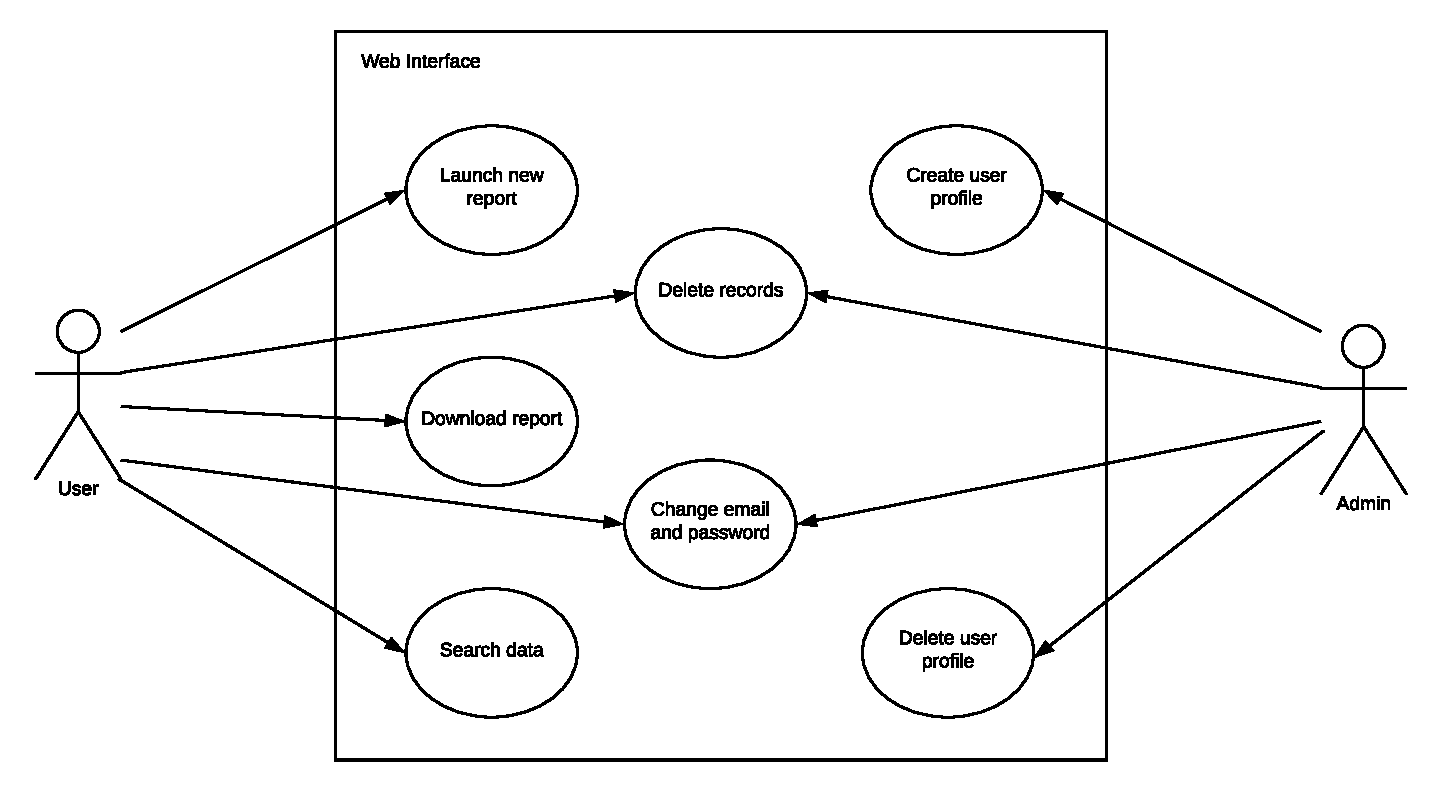
\includegraphics[scale=0.6]{imgs/UseCasesDiag.pdf}
\caption{Use cases diagram}
\label{fig:usecases}
\end{figure}

The figure provides a simplified set of possible actions, with no regard to the
exact order in which they may be presented to the user under realistic
circumstances. Use-cases are a schematic way to visualize the main functions of a
system from the users' perspective.

The following set of tables will flash out what each use-case requires and what
provides:

\begin{table}[H]
\centering
\begin{tabular}{l p{9cm}}  
\toprule
\bf{Use case name}    & Launch new report \\
\midrule
\bf{Actor}    & Investigator \\
\midrule
\bf{Description}    & The user selects the type of report he/she wants to
generate, fills in the necessary input and submits the request. \\
\midrule
\bf{Preconditions}    & The user has to be logged into his/her profile. \\
\midrule
\bf{Trigger}    & Click on \emph{Submit} button. \\
\bottomrule
\end{tabular}
\caption{Launch new report use case}
\end{table}

\begin{table}[H]
\centering
\begin{tabular}{l p{9cm}}  
\toprule
\bf{Use case name}    & Delete records \\
\midrule
\bf{Actor}    & Investigator, Admin \\
\midrule
\bf{Description}    & The user deletes records associated with a case. \\
\midrule
\bf{Preconditions}    & The user has to be logged into his/her profile. \\
\midrule
\bf{Trigger}    & Click on \emph{Delete} icon. \\
\bottomrule
\end{tabular}
\caption{Delete records use case}
\end{table}

\begin{table}[H]
\centering
\begin{tabular}{l p{9cm}}  
\toprule
\bf{Use case name}    & Create user profile \\
\midrule
\bf{Actor}    & Admin \\
\midrule
\bf{Description}    & The user create a new profile with a username, email and
password that will allow a new user to access the system functionalities.
\\
\midrule
\bf{Preconditions}    & The user has to be logged into his/her profile. \\
\midrule
\bf{Trigger}    & Click on \emph{Save} button. \\
\bottomrule
\end{tabular}
\caption{Create user profile use case}
\end{table}

\begin{table}[H]
\centering
\begin{tabular}{l p{9cm}}  
\toprule
\bf{Use case name}    & Download report \\
\midrule
\bf{Actor}    & Investigator \\
\midrule
\bf{Description}    & The user selects a report that has already been
generated, and downloads a csv file with the data.
\\
\midrule
\bf{Preconditions}    & The user has to be logged into his/her profile. Data
from a report has to be already available and saved in the database.
\\
\midrule
\bf{Trigger}    & Click on \emph{Download} icon. \\
\bottomrule
\end{tabular}
\caption{Download report use case}
\end{table}

\begin{table}[H]
\centering
\begin{tabular}{l p{9cm}}  
\toprule
\bf{Use case name}    & Change email and password \\
\midrule
\bf{Actor}    & Investigator, Admin \\
\midrule
\bf{Description}    & The user can change the current password and email
address.
\\
\midrule
\bf{Preconditions}    & The user has to be logged into his/her profile.
\\
\midrule
\bf{Trigger}    & Click on \emph{Save} button. \\
\bottomrule
\end{tabular}
\caption{Change password use case}
\end{table}

\begin{table}[H]
\centering
\begin{tabular}{l p{9cm}}  
\toprule
\bf{Use case name}    & Search data \\
\midrule
\bf{Actor}    & Investigator \\
\midrule
\bf{Description}    & The user can submit a set of keywords and find out how
many reports are available in the database associated with that term.
\\
\midrule
\bf{Preconditions}    & The user has to be logged into his/her profile.
\\
\midrule
\bf{Trigger}    & Click on \emph{Search} button. \\
\bottomrule
\end{tabular}
\caption{Search use case}
\end{table}

\begin{table}[H]
\centering
\begin{tabular}{l p{9cm}}  
\toprule
\bf{Use case name}    & Delete user profile \\
\midrule
\bf{Actor}    & Admin \\
\midrule
\bf{Description}    & The user can delete the profile of a user that no longer
needs access to the system.
\\
\midrule
\bf{Preconditions}    & The user has to be logged into his/her profile.
\\
\midrule
\bf{Trigger}    & Click on \emph{Delete} button. \\
\bottomrule
\end{tabular}
\caption{Delete user profile use case}
\end{table}

\section{Requirements}
I already mentioned some of the requirements and system constraints in the
\emph{system architecture} section. In this section I will discuss in more
details all the requirements considered for the current implementation.
Requirements are further divided in functional, non-functional and user
requirements.

\subsection{Functional requirements}
Functional requirements concern the core business logic of the system:
\begin{description}
\item[F1] the system should connect successfully to external sources, public
API, to retrieve relevant data.
\item[F2] The system should collect data extracted from external sources and
store it in a local database.
\item[F3] The system should avoid storing duplicates of the same record within
one report request.
\item[F4] The system should assemble all the data gathered for one user's
request and print it in a csv file format.
\item[F5] The system should send a copy of the data, to the requesting user, in
a csv file attached to a notification email.
\item[F6] The system should limit the amount of API calls to each external data
source, in order not to breach API user policy.
\end{description}

\subsection{Non-functional requirements}

\begin{description}
  \item[N1] The system should restrict access to authorized users only.
  \item[N2] The system should store users' passwords encrypted.
  \item[N3] The system should store data gathered from external sources
  encrypted while the data is at rest.
  \item[N4] The system should be hardened against most common web attacks.
  \item[N5] The system should be prepared to accommodate larger data
  sets;
  \item[N6] The system should be prepared to accommodate more web servers to
  increase performance, redundancy and fault-tolerance.
  \item[N7] The database should allow flexible storage of heterogeneous
  data-schemes from different sources.
\end{description}

\subsection{User requirements}
\begin{description}
\item[U1] The application should allow access to the authenticated user.
\item[U2] The user should be able to change his/her password and email.
\item[U3] The application should present the list of all queries run by the user
in the last two weeks.
\item[U4] The application should allow the user to search and filter through
his/her cases based on case creation date range and platform (e.g. eBay,
MercadoLibre, Allegro, Facebook, etc.).
\item[U5] The application should provide input-forms to allow data extraction
from all the external data sources available.
\item[U6] The application should preform data gathering operations without
stopping the user from performing other operations.
\item[U7] When the data is ready to download the user should be notified.
\item[U8] The user should be able to access both data and input provided for old
cases.
\item[U9] The user should be able to delete old cases and data associated with
them.
\end{description}

\section{Class diagram}
The class diagram in figure \ref{fig:clssdiag} represents the core modules of
the web application.

Django provides three parent classes that represent web-forms, html page
generators and data base tables called respectively: Forms, Views and Models.
These classes can be inherited to produce specific objects to fit the needs of
the project.

The \texttt{Forms} class for instance offers default fields that represent the
values of its fields (e.g. text fields, date fields, numeric fields\ldots), and methods
that allow data sanitization, html layout, data validity. Linkero inherits this
class to produce the \texttt{CaseFilerForm}, which is a simple form that enables
users to limit the amount of cases to be displayed on the main page, by
selecting a time range and a platform (e.g. show only cases from Jan to Feb
2018, that pulled eBay data). The \texttt{CaseFilerForm} object was created by declaring
the list of fields that should be part of the form, all other methods were
inherited from the parent class.

The \texttt{Models} class is the core of Django's ORM (Object Relational Mapping)
philosophy: it is a Python object that maps its fields to a database table (or
document in MongoDB's case), and offers as many methods as SQL or NoSQL
functions to read and write data. Like for Forms, the Models parent class
provides all the methods that are needed, while the developer is left with
declaring the field types for each object. In this project, the
\texttt{CaseDetails} model represents information about a specific case: the
case identification number, the creation date, the case owner, the platform which
sourced the data, the inputs provided for the data search. Similarly the model
\texttt{EbayItem} stores all the information about an eBay item that was queried
and stored in MongoDB.

The \texttt{Views} class represents the objects that receives a http request and
returns a response. Each child class will have their own implementation of one
or both GET and POST methods. The class \texttt{CaseView} for instance represents the
home page being displayed after the user logs in: a table that summarizes all
the cases generated in the last two weeks, and a menu to bring up modal forms to
submit new data requests. The GET method detects when it is receiving a
request to load the full page, or an AJAX GET request to load just a new
filtered set of cases in the cases table. The POST method of the
\texttt{CaseView} class receives requests to generate new reports.

The last class in the diagram is \texttt{EbayAPI}. This class does not inherit
from any other built-in Django object. Instead it was created from scratch to
provide querying facility with eBay public APIs. Its fields represent
authentication details for the local database and the remote server, whereas its
methods are designed to extract data based on user's input, leveraging eBay
APIs like general search by keyword, get details by item number or get seller
details by seller id.

The diagram indicates also classes' level of coupling, or how much a modules
shares data and interacts with other modules. Forms and Views are in one-to-one
relations most of the time, since forms are unique, and each view incorporates
one form for each type. Models and Views instead are in many-to-one relations,
since each view can interact with multiple instances (i.e. database records)
from the same class, but there is always only one view object at any given time.

\begin{figure}[H]
\centering
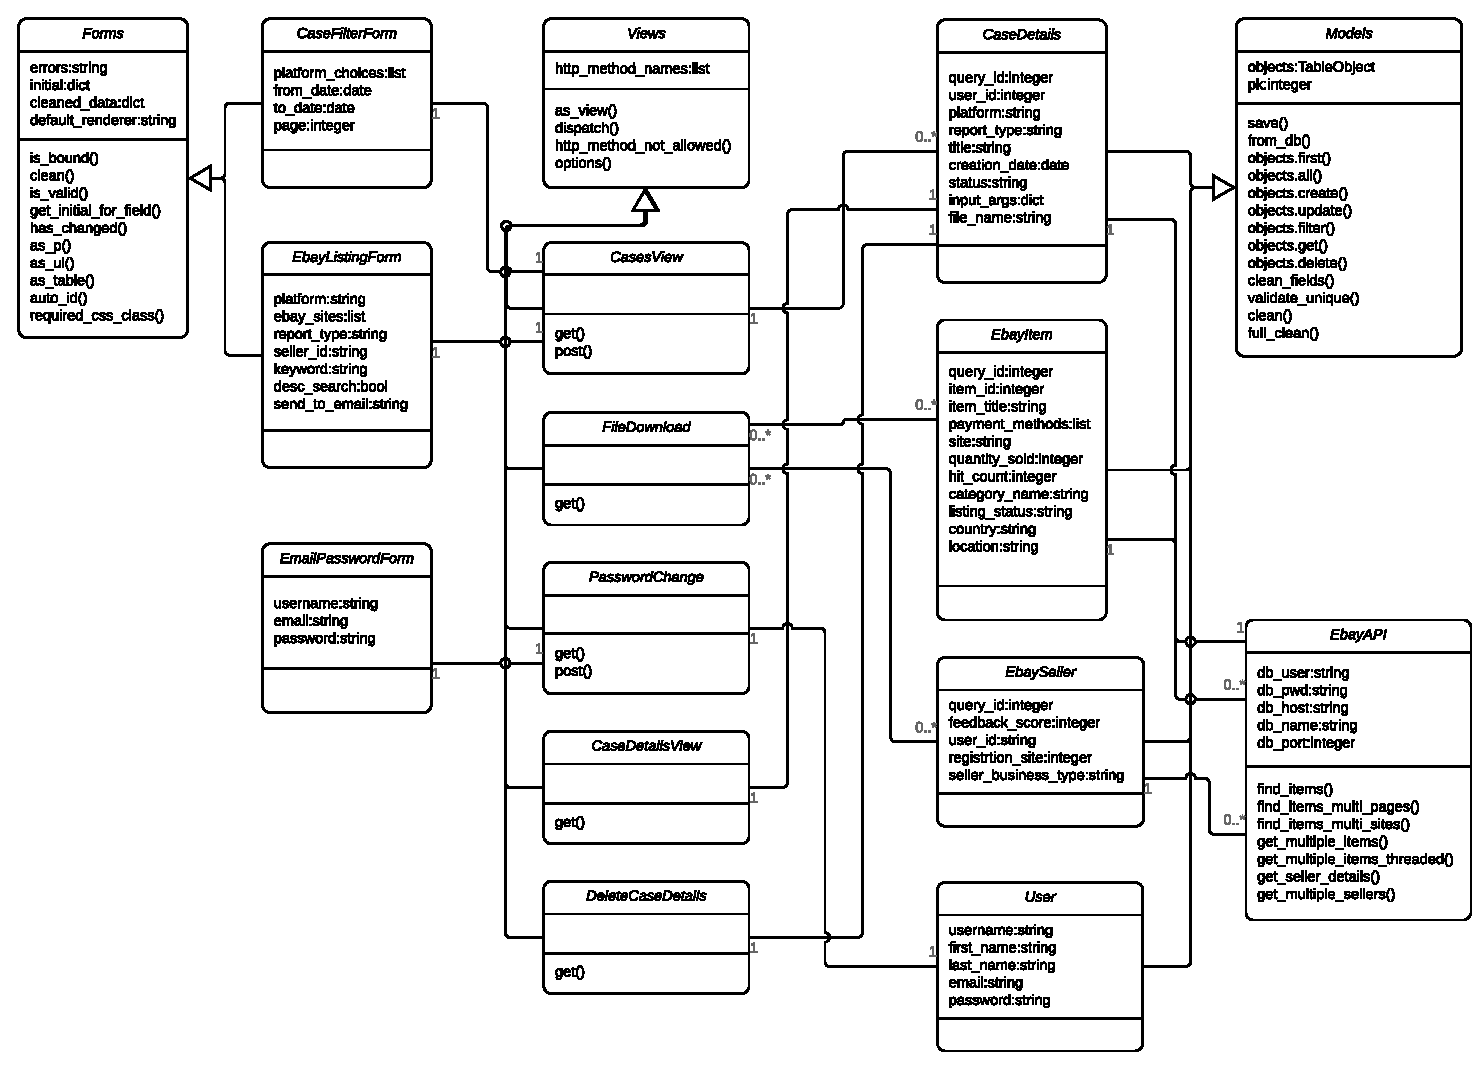
\includegraphics[angle=90, scale=0.9]{imgs/ClassDiag.pdf}
\caption{Class diagram}
\label{fig:clssdiag}
\end{figure}

\section{Sequence diagram}
The sequence diagram represented in figure \ref{fig:sqncdiag} is probably the
most elaborate process performed by the core business logic in Linkero. It
describes the sequence of operations that the system performs after receiving a
request to generate a new report.

The entire sequence can be broken down into the following steps:
\begin{enumerate}
\item The process is triggered by the user submitting a POST request through a web-form
designed to gather all necessary input to pull data from external
resources.
\item The \texttt{CaseView} object receives the request and immediately saves
the details of the new case in the database by making a call to the
\texttt{CaseDetails} object and using the \texttt{save()} method. The case
details are saved and nothing is returned, assuming there are no errors or
exceptions raised.
\item Next, the \texttt{CaseView} instance submits a report
request to the \texttt{Task} controller, the controller queues the request
and returns the call to \texttt{CaseView} instance that in turn can send a
response back to the client browser that initiated the process, confirming that
the request for a new report was successfully submitted.
\item The \texttt{Task} controller script continues the process
asynchronously by requesting the \texttt{EbayAPI} to pull a list of items.
\item The \texttt{Task} receives the results and saves them with the
\texttt{save()} method of the \texttt{EbayItems} object.
\item The \texttt{Task} controller proceeds to request details of the sellers
extracted from the previews search by calling the \texttt{search\_sellers()}
method of the \texttt{EbayAPI} object.
\item The results are then saved by the \texttt{EbaySellers} object.
\item Once the data necessary to generate a new report is ready, the
\texttt{Task} script creates a new .csv file and parses the results there.
\item The \texttt{Task} controller sends the data to the EmailServer objects
that is responsible for sending an email notification to the user who requested
the report.
\item Finally, the \texttt{Task} controller changes the status of the request
from \emph{running} to \emph{completed} by using the \texttt{update\_status()}
method of the \texttt{CaseDetails} instance.
\item While all other objects remains ready to answer calls, the \texttt{Task}
script ends its cycle.
\end{enumerate}

\begin{figure}[H]
\centering
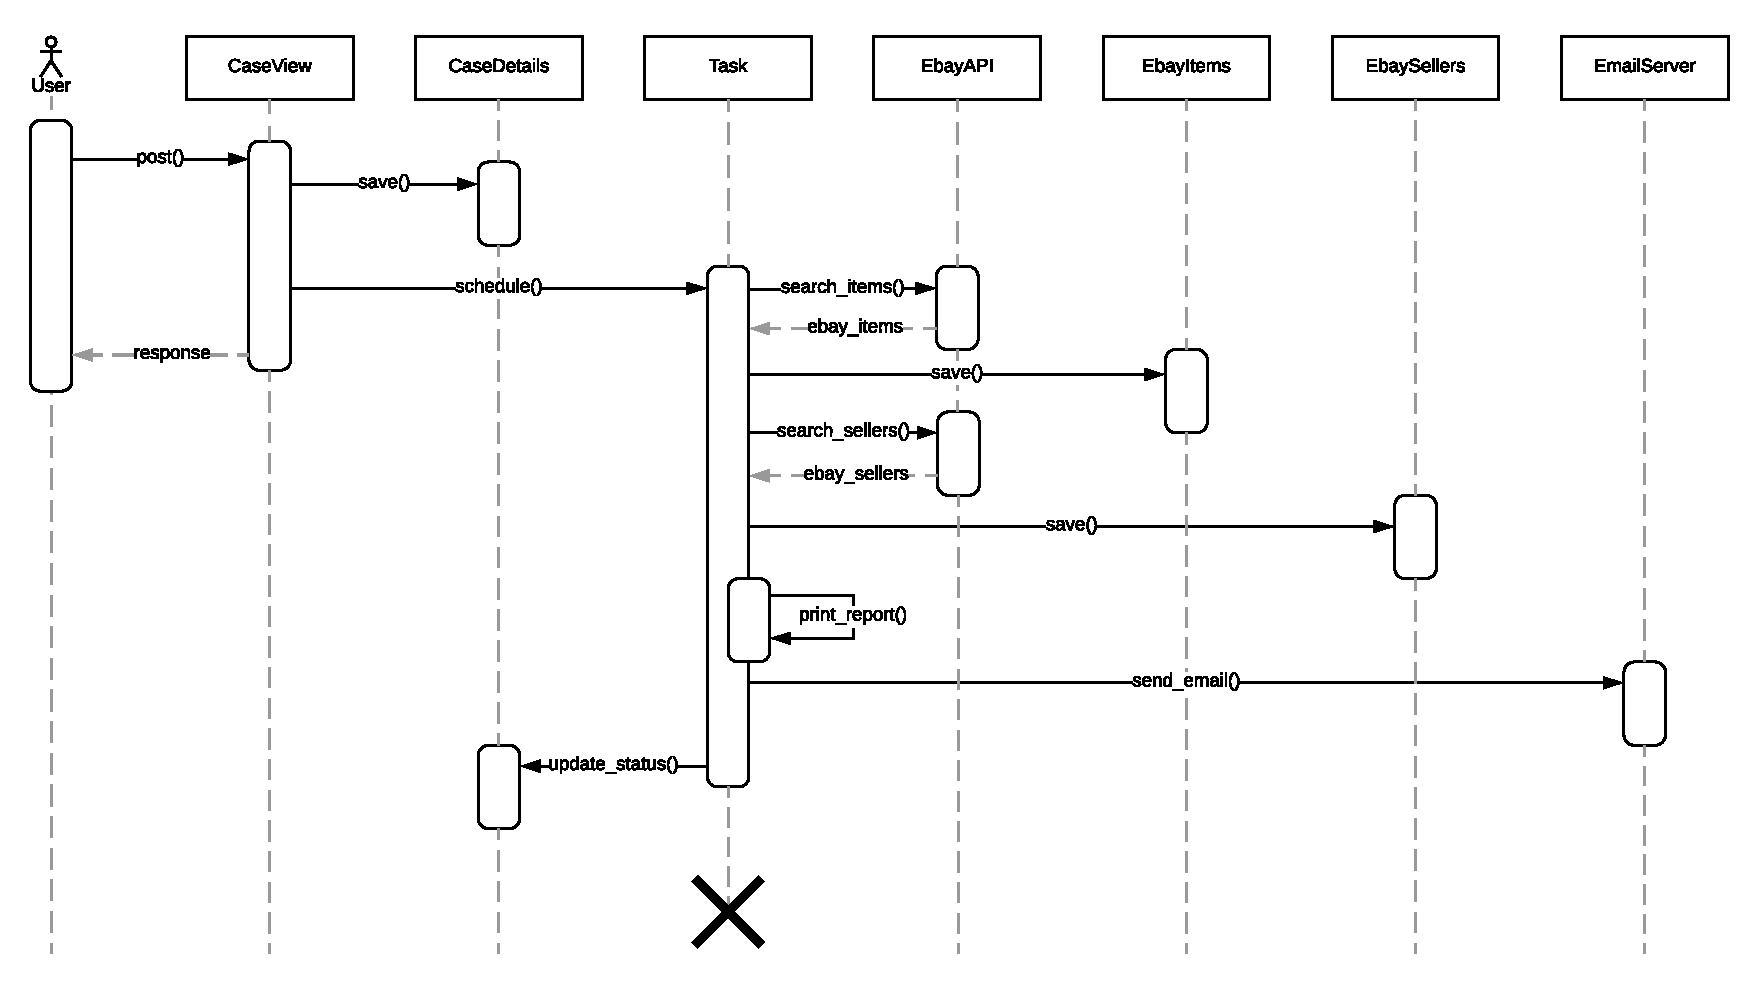
\includegraphics[angle=90, scale=0.6]{imgs/SequenceDiagram.pdf}
\caption{Launch report sequence diagram}
\label{fig:sqncdiag}
\end{figure}

\section{Code samples}
In this section I will look at some code snippets that make up the
\texttt{Task} script just described in the sequence diagram.

The first part of the script is dedicated to load necessary libraries of
function that support the script execution, including the \texttt{EbayApi}
object, and the models connected with the MongoDB database:
\begin{lstlisting}[language=Python, breaklines=true]
import os
import time
import json
from csv import DictWriter
from io import StringIO
from celery import task
from pandas import merge
from pandas.io.json import json_normalize
from mongoengine import connect
from django.contrib.auth.models import User
from django.core.mail import EmailMessage
from cases.ebayapi import EbayApi
from cases.models import EbayItem, EbaySellerDetails, ApiErrorLog, CaseDetails
\end{lstlisting}

Immediately after the task process is declared:
\begin{lstlisting}[language=Python, breaklines=true]
def send_ebay_listing_report(to_email, user_id=None, query_id=None,
seller_id=None, keywords=None, ebay_sites=['US'], search_desc=False):
\end{lstlisting}

In the following lines I create a connection to MongoDB, so that instances
representing its collections (read tables) will be able to retrieve and store
data in them, and I initiate an EbayApi instance:
\begin{lstlisting}[language=Python, breaklines=true]
    # connect to Mongo
    mongo_client = connect('linkerodb', username='linkero-user',
    password='password123')
        
    ea = EbayApi()
\end{lstlisting}

The script then uses the \texttt{find\_items\_multi\_sites()} method of the
\texttt{EbayApi} instance to search and pull all items that match the criteria
input by the user. If the search returns results, the script continues to
generate the report, otherwise it jumps to a last step sending a notification
to the user that no items were found:
 \begin{lstlisting}[language=Python, breaklines=true]
    items_dict, slr_list, find_error_list = ea.find_items_multi_sites(e_sites=ebay_sites, kwd=keywords, s_id=seller_id, s_desc=search_desc)
    
    # check if find items search returned results
    if items_dict:
\end{lstlisting}

Assuming that the first exploratory search was successful, the script proceeds
to pull the details for each item, and subsequently the business details for
each seller:
\begin{lstlisting}[language=Python, breaklines=true]
		# pull item descriptions for each item
		ebay_item_list = ea.get_multi_items_threaded(items_dict, q_id=query_id)
        
        # pull seller details
        seller_list, seller_err_list = ea.get_multiple_sellers(seller_list=slr_list)
        seller_collection_list = []
        for slr in seller_list:
            slr['lnkr_query_id'] = query_id
            seller_collection_list.append(EbaySellerDetails(**slr))
        # insert in bulk
        EbaySellerDetails.objects.insert(seller_collection_list)
\end{lstlisting}
Probably not the most consistent class design implementation, but in the case of
the \texttt{EbayApi} instance method \texttt{get\_multi\_items\_threaded()},
items are saved in the corresponding MongoDB collection by the \texttt{EbayApi}
instance itself; while seller details are retrieved by the \texttt{EbayApi} and
passed back to the \texttt{Task} script in memory, and it is the \texttt{Task}
script that calls the database object \texttt{EbaySellerDetails} to save the
details retrieved. This \emph{double standard} was implemented after a series of
tests, when I found that leaving the data in the \texttt{Task} script memory
would cause memory overflow and the script would crash. It is worth to remember
that the system that is currently running this project only has 1GB of memory.

Continuing, the data extracted is then assembled into a csv file:
\begin{lstlisting}[language=Python, breaklines=true]
        # save the results in a CSV file and send it attached
        e_items = EbayItem.objects(lnkr_query_id=query_id)
        items_df = json_normalize(json.loads(e_items.to_json()))
        
        sellers_df = json_normalize(seller_list)
        
        df = merge(items_df, sellers_df, left_on='Seller.UserID', right_on='UserID')
        
        filename = "linkero_ebay-listings_{}.csv".format(time.strftime("%Y%m%d-%H%M"))
\end{lstlisting}

In order to save system hard-disk space, the script creates a file-like object
\texttt{StringIO} that is compatible with Python file manipulation API,
but is never committed to permanent storage:
\begin{lstlisting}[language=Python, breaklines=true]
        file_attachment = StringIO()
        writer = DictWriter(file_attachment, fieldnames=headers)
        writer.writeheader()
        writer.writerows(df.to_dict('records'))
        file_attachment.seek(0)
        email.attach(filename, file_attachment.read(), 'text/csv')
        email.send(fail_silently=False)
        file_attachment.close()
        
        # update the case execution status
        query_status = 'completed'
        CaseDetails.objects(lnkr_query_id=query_id).update(set__file_name=filename)
\end{lstlisting}
The last line calls the MongoDB instance dedicated to case details,
\texttt{CaseDetails}, and changes the status of the report from \emph{running}
to \emph{completed}.

The full code of the Django application is available at
\url{https://github.com/srichiardi/linkero}.
\vfill


\section{Front end screenshots}

\begin{figure}[H]
\centering
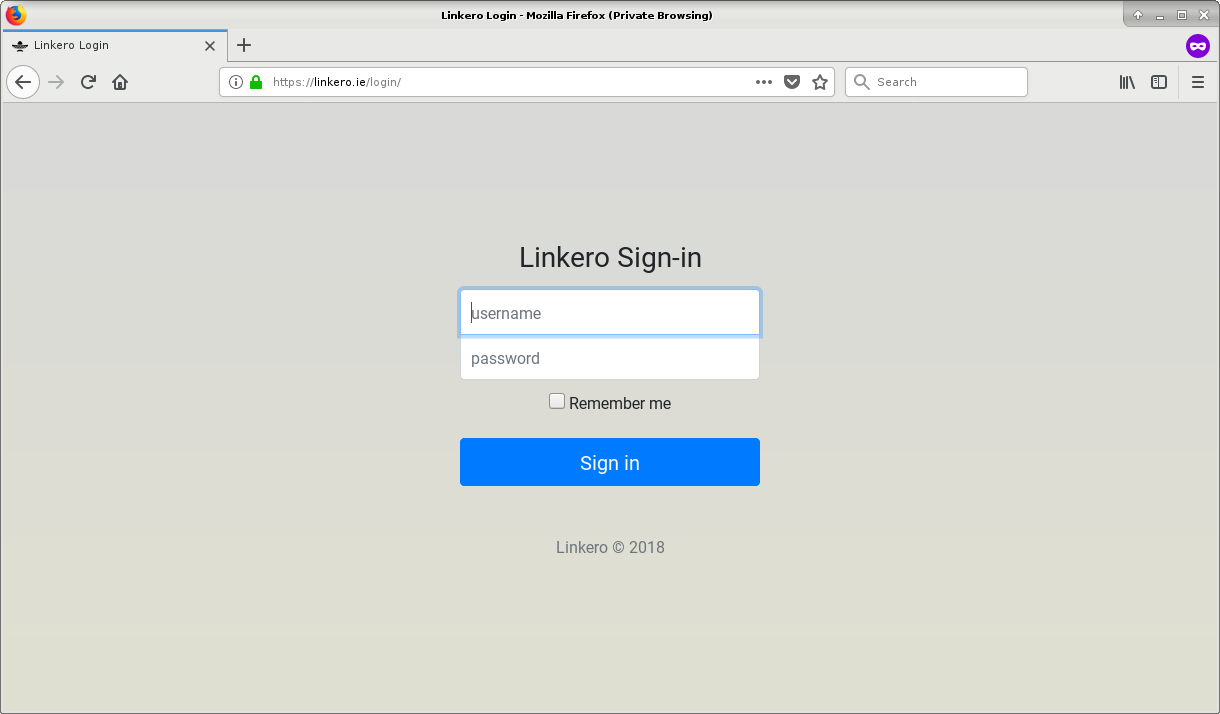
\includegraphics[scale=0.3]{imgs/login.png}
\caption{Login page}
\label{fig:login}
\end{figure}

\begin{figure}[H]
\centering
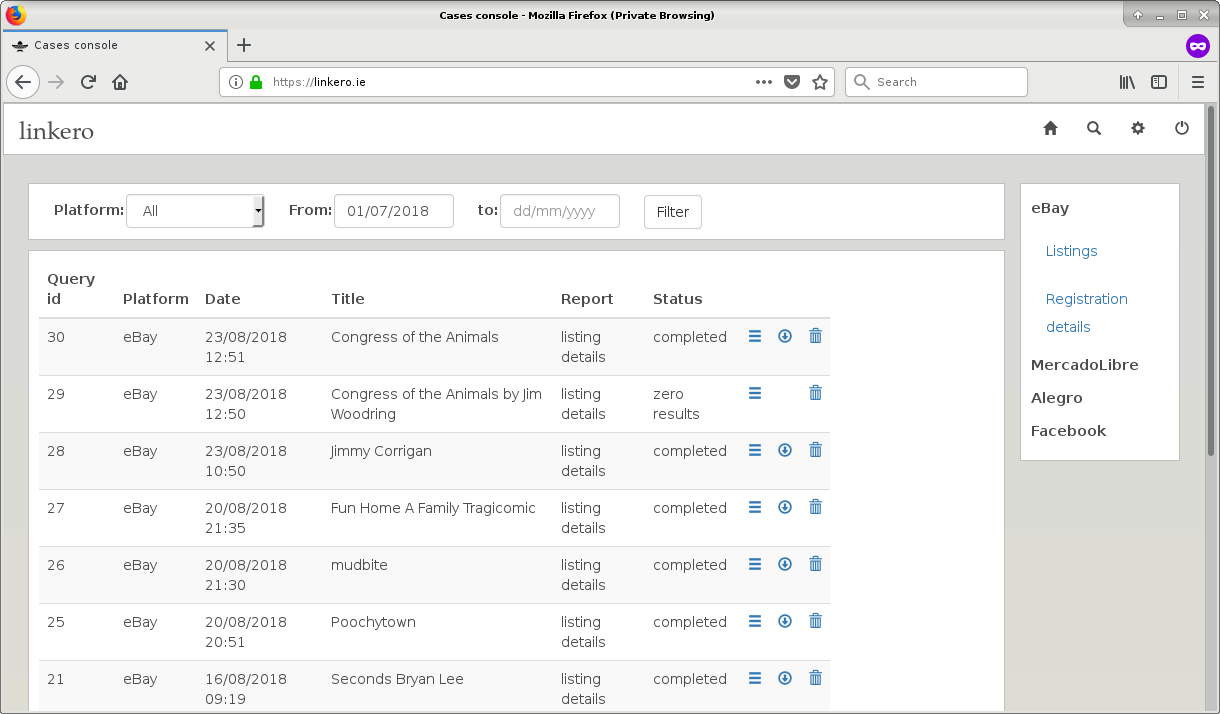
\includegraphics[scale=0.3]{imgs/HomeScreen.png}
\caption{Home page}
\label{fig:home}
\end{figure}

\begin{figure}[H]
\centering
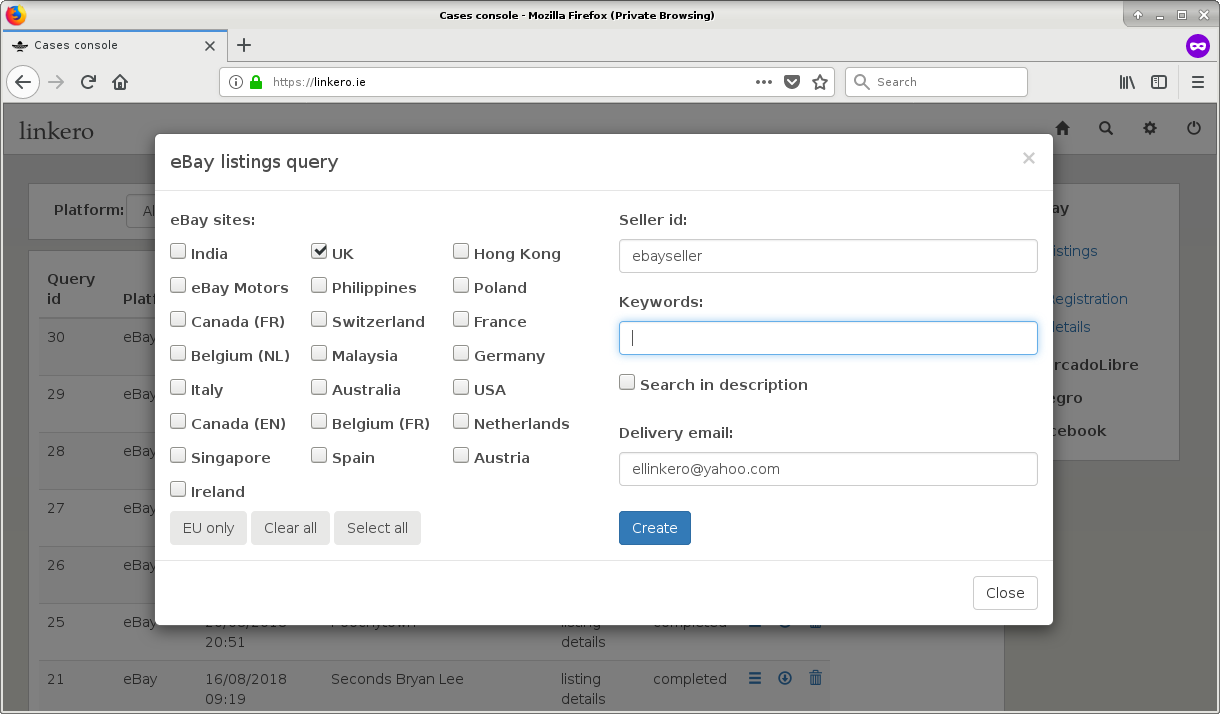
\includegraphics[scale=0.3]{imgs/InputForm.png}
\caption{eBay input modal form}
\label{fig:inputform}
\end{figure}

\begin{figure}[H]
\centering
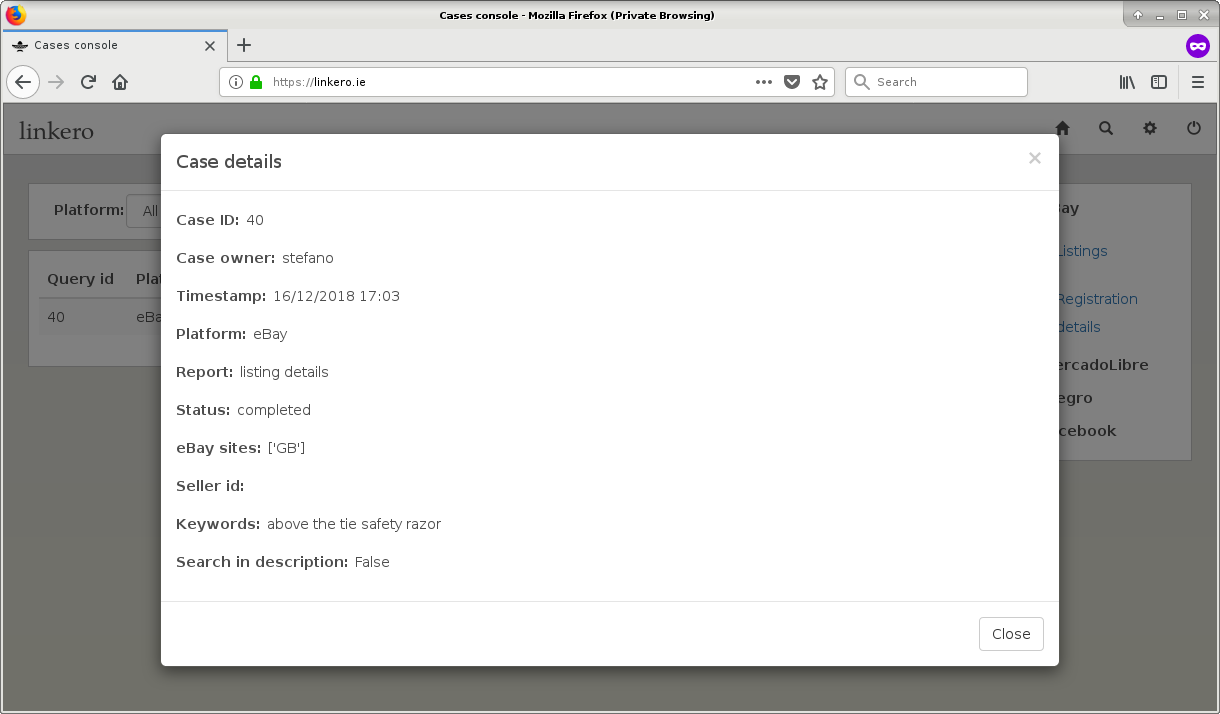
\includegraphics[scale=0.3]{imgs/case_details.png}
\caption{Case details modal}
\label{fig:casedetails}
\end{figure}

\begin{figure}[H]
\centering
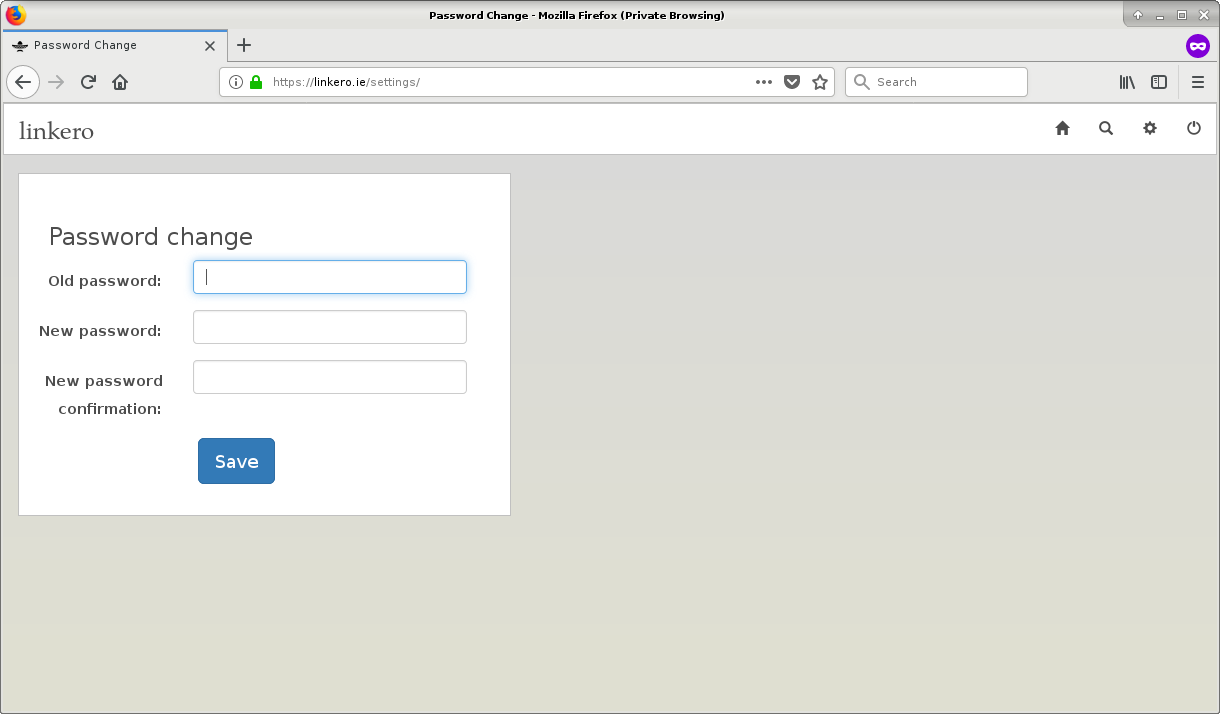
\includegraphics[scale=0.3]{imgs/PasswdChange.png}
\caption{Password change form}
\label{fig:pwdform}
\end{figure}

